\documentclass[20pt,margin=1in,innermargin=-4.5in,blockverticalspace=-0.25in]{tikzposter}
\geometry{paperwidth=42in,paperheight=30in}
\usepackage[utf8]{inputenc}
\usepackage{amsmath}
\usepackage{amsfonts}
\usepackage{amsthm}
\usepackage{amssymb}
\usepackage{mathrsfs}
\usepackage{graphicx}
\usepackage{adjustbox}
\usepackage{enumitem}
\usepackage[backend=biber,style=numeric]{biblatex}
\usepackage{emory-theme}
\usepackage{url}
\usepackage{graphicx}

\usepackage{mwe} % for placeholder images

\addbibresource{refs.bib}

% set theme parameters
\tikzposterlatexaffectionproofoff
\usetheme{EmoryTheme}


\title{Main Locations Extraction in Literature}
\author{Ohad Edelstein, Nitzan Katz}
\institute{IDC, Israel}

% begin document
\begin{document}
\maketitle
\centering
\begin{columns}
    \column{0.32}
    \block{Abstract}{
        The purpose of this project is to extract the locations related to main characters in books. This may contribute to a bigger task of making a site-seeing route based on the route of main characters in archaeology books. The project includes POS (part of speech) tagging and NER (name entity recognition) in books, characters relational graph based on sentiment analysis and characters-locations co-occurrences graph. We mostly rely on commonly used models for solving this issue rather than inventing new models for the specific tasks.
    }
    \block{The Problem in More Details}{
          The issue of narative extraction in books is still a big problem in the field of NLP. As this complicated task is right now, it can be put down to smaller easier problems to solve. Some of those tasks include main characters extraction and the places the plot takes place in. Those two tasks are the ones we scoped in in this project. The solution icludes many common NLP aspects, as POS tagging for finding names in texts, NER for characters and locations extractions. The main added value of this project is the examination of the relations between the characters and the locations. There's no common way in solving this task and the method presented in this project can be a valid approach for this problem and shows some interesting results.
    }
    \block{Method}{
        In our work\cite{project2020} we took a similar approach as taken in an existing project\cite{hzjken2019char}, where characters were extracted from a Harry Potter book using SpaCy\cite{spacy} pre-trained models. After that, a co-occurrence matrix to describe the relations between the characters. The weight of the relation is calculated by the amount of times two characters appeared in the same sentence in the book. Besides that, a sentiment matrix is calculated by testing the affinity of each sentence two characters appeared in. This can show us the nature of the relationship rather than just how common the connection is. Our idea was based on the co-occurrence matrix, and used that concept to extract the main character. The main difference is that on top of that, we extracted the locations in the same way, and we also calculated a co-occurrence matrix for the characters with the locations to see the locations the main characters are related to. This might show us the main locations in the book based on the main characters which are supposed to be the base for the plot of the book.
    }

    \column{0.36}
    \block{Results}{
        At first, we recreated the results shown in the project. For that we cloned the project and mostly ran it as it is. We also downloaded the relevant Harry Potter books to see if it works. The results were identical to what shown in the project, so we kept with the idea. After that we extracted the locations out of the book. For that, we looked into the SpaCy models, and used the relevant labeling for locations. The labels "GPE", "LOC" and "FAC" are our indication of places in the book. The locations we found in Harry Potter: Sorcerer's Stone were pretty interesting. The list we got is: 'firenze', 'london', 'flint', 'romania', 'privet drive', 'uncle vernon', 'smelting stick'. Which contains both real locations, like firenze, and london, but also misfits from the algorithm, like privet drive or uncle vernon. However, only the real locations receive a serious enough relation to be noticeable in the graph itself (There are connections between some of the other characters and locations, it's too low to be seen as the strength of the color is determined by the amount of co-occurrences). We also had some issues with names there were mis-interpreted as locations, which we removed later if they were labeled as both names and locations (we decided to include them as just names). To calculate the relations between the locations and the characters we basically combined the names and the locations after the most common names and locations were filtered and used the same matrix creation as before. Then we only use the results regarding the relations between the parts of the names with the parts of the locations.
        
        After we had these results on the Harry Potter book, we wanted to see on a non-fiction world based book to see what results we will receive. We chose Clancy Tom's book "Patriot Games" and created a generic notebook that does the whole process given the path to the book's file. Since the project we were based on only checked the algorithm on Harry Potter books now it's also interesting to see the co-occurrence graph and see the relations between the characters. From the relations graph we can see the main character Jack Ryan as the characters with most strong connections (Jack), also with Cathy which is Jack's wife and also a main character and Sally, his daughter. All three of them have the last name Ryan which is also shows as main in here which makes sense.
        
        Since the relations graph makes sense, we continued for the characters-locations relations graph. The results are pretty interesting (figure 1) the main locations are London, America, Baltimore, Annapolis and Washington which are indeed related to the plot of the story. Notice that there's a strong connection between Sergeant and Highland, when we're not familiar in detail with the book we can't make sense of a location name Highland on it's own. It might be another main location, and it might be an outlier.
        \begin{tikzfigure}[Clancy Tom Patriot Game Locations Graph]
            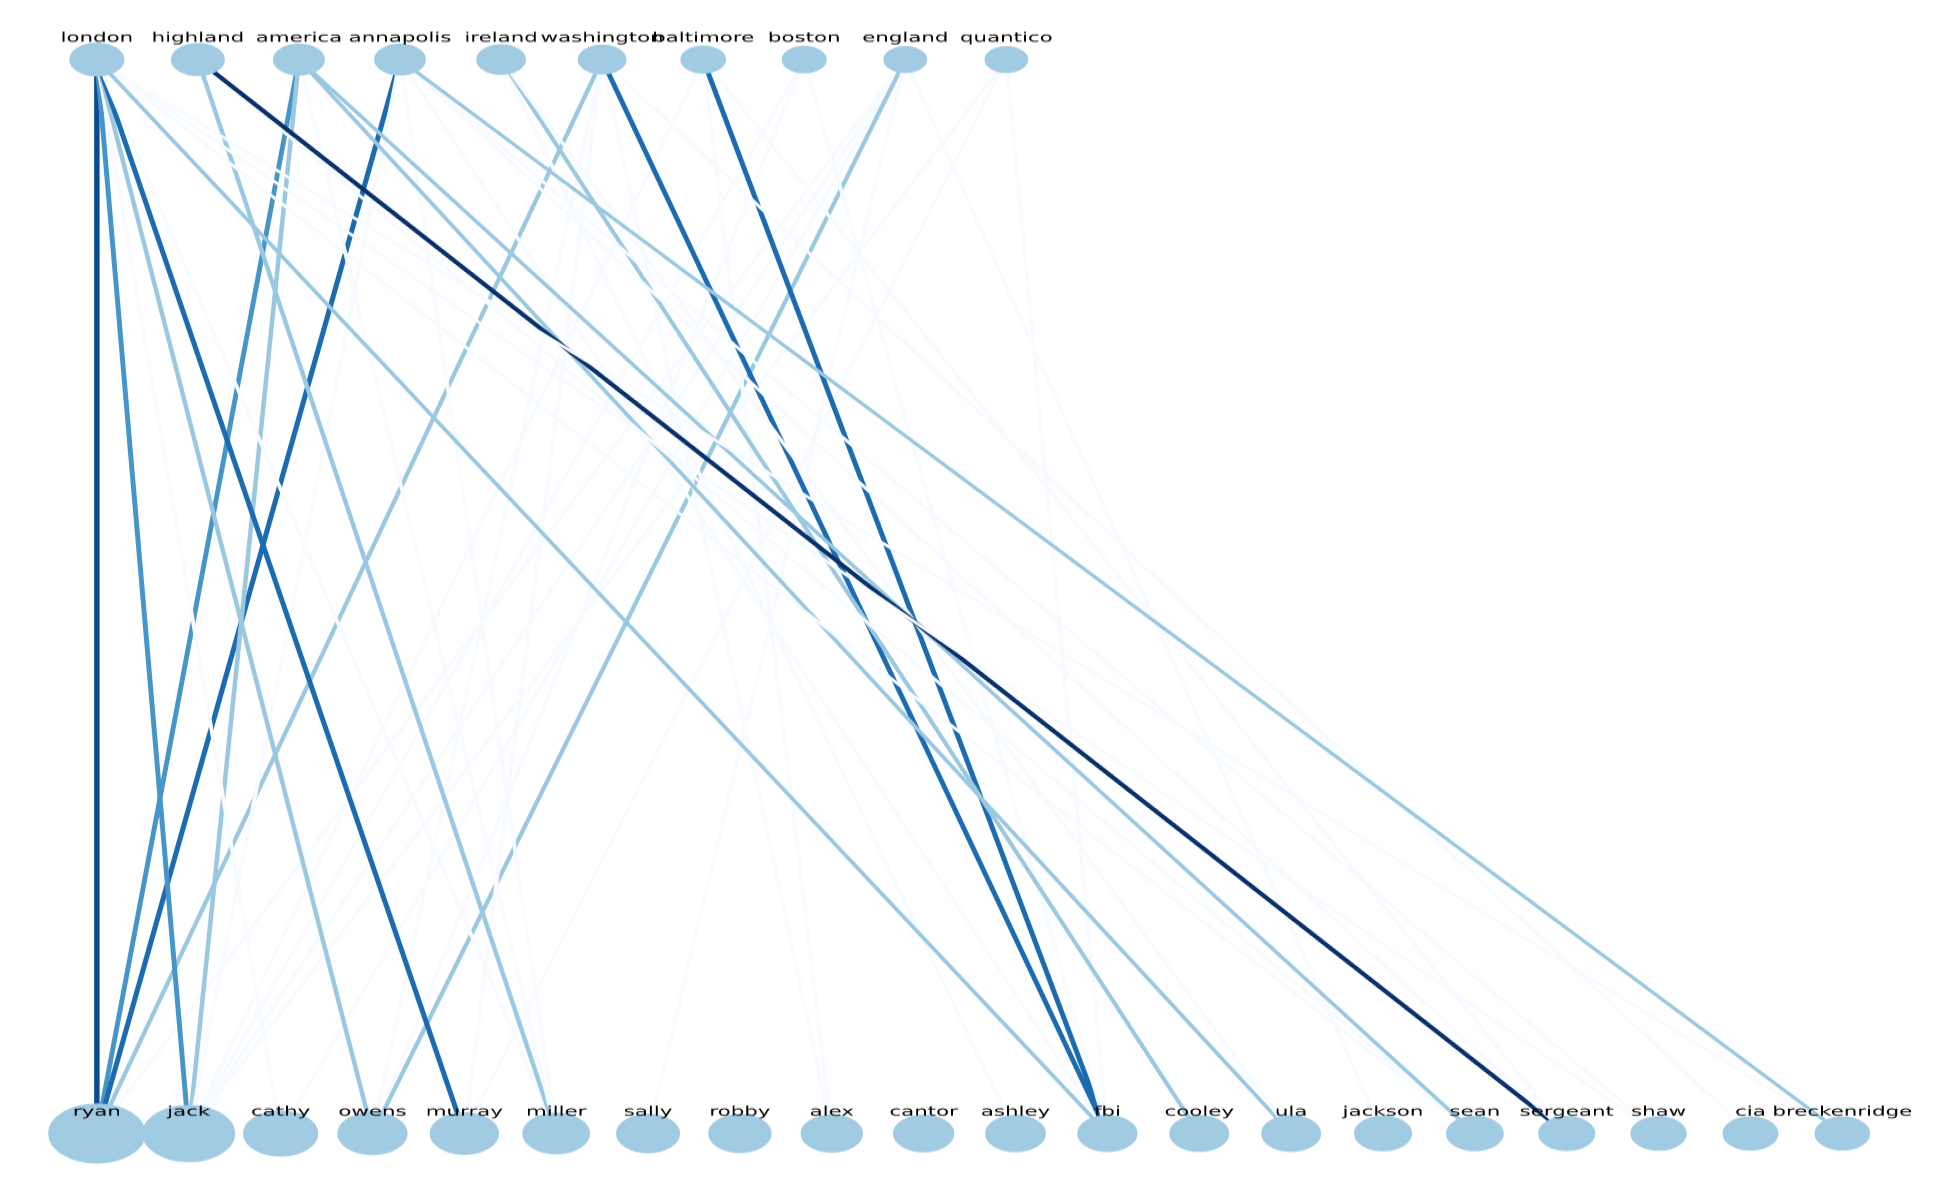
\includegraphics[height=0.16 \textwidth]{Tom Clancy - Patriot Games locations graph.png}
        \end{tikzfigure} 
        Either way, this graph shows pretty good results as a proof-of-concept for the idea, where the next stage would be comparing the model's results to tagged archaeology books and see the matching rate.
        
    }

    \column{0.32}
    
    \block{Conclusions}{
        The results shown here are primal, and further examination on a variety of novels is required to make any reliable point. There are still more directions that can be investigated and might lead to better and more reliable results, some of them are as follows.
        \begin{itemize}
            \item Changing the co-occurrence method - We basically only looked at words that appeared in the same sentence as related words. Other scopes, such as a whole paragraph or even few following sentences might lead to more connections between certain characters and locations and better focus the main aspects of the book than the current method.
            \item Relations to references - The method used above only takes names into account and totally ignores more complicated references to them like "he", "she", "they" and so on... This causes a major lack of relational information as characters are usually referred to by those words and not by their name every time.
            \item Full names - As part of the solution, full names are split into first and last names and are counted separately, though it has it advantages, as it combines references to the same character even when it is mentioned differently, it also causes unwanted combination of characters (as few family members will all appear with the same last name), and also leads to split in the references of the same character (if the character sometimes referred to by its first name and sometimes by its last name). A technique to overcome this obstacle needs to be carefully examined to work properly.
        \end{itemize}

        However, this proof-of-concept shows that this direction do have a good point and should be taken into farther research to get to its full potential.
        }
                
    \block{References}{
        \vspace{-1em}
        \begin{footnotesize}
        \printbibliography[heading=none]
        \end{footnotesize}
    }
\end{columns}
\end{document}